\documentclass[12pt]{article}
\usepackage{amssymb}
\usepackage{geometry}
\usepackage{listings}
\usepackage{graphicx}
\usepackage{amsmath}
\usepackage{wrapfig}
\usepackage{amsmath}
\usepackage{lipsum}
\usepackage{caption}
\usepackage{ulem}
\usepackage{xcolor}
\usepackage{tikz}
\usetikzlibrary{arrows.meta, positioning, shapes}

\usepackage{sectsty}
\sectionfont{\color{sectionColor}}       % Color for \section
\subsectionfont{\color{subsectionColor}}


\definecolor{titleColor}{HTML}{800000}        % Maroon
\definecolor{sectionColor}{HTML}{4682B4}      % SteelBlue
\definecolor{textHighlight}{HTML}{DAA520}     % Goldenrod
\definecolor{backgroundColor}{HTML}{F0F8FF}   % AliceBlue
\definecolor{emphasisColor}{HTML}{228B22}     % ForestGreen
\definecolor{subsectionColor}{HTML}{6A5ACD}   % SlateBlue


\title{\textcolor{titleColor}{\textbf{\Huge \textbf{ Monte Carlo Simulation Report\\
Recovery of War-Affected Medical Students in Sudan }}}}

\author{B. M. Lyla\thanks{Al Khartoum University, Faculty of medicine  Cairo \\ \texttt{lylababiker@gmail.com}}}
\date{\today}
\begin{document}
\maketitle


\section*{Introduction}
This report presents the results of a Monte Carlo simulation for 100 medical students affected by war in Sudan. 
The students are categorized into three groups: \textbf{Trauma}, \textbf{Stress and Anxiety}, and \textbf{Depression}.
Each group is assigned a doctor and follows a recovery protocol.

\section*{Simulation Parameters}
\begin{itemize}
  \item Number of students: 100
  \item Number of simulations: 1,000 iterations
  \item Recovery probabilities:
  \begin{itemize}
    \item Trauma: 60\%
    \item Stress and Anxiety: 75\%
    \item Depression: 50\%
  \end{itemize}
\end{itemize}



% Listings settings
\lstset{
  basicstyle=\ttfamily\small,
  numbers=left,
  numberstyle=\tiny,
  breaklines=true,
  frame=single,
  columns=fullflexible,
  keywordstyle=\color{blue},
  commentstyle=\color{gray},
  stringstyle=\color{orange},
  showstringspaces=false
}


\section*{Python Simulation Code}

Below is the Python script used to simulate recovery for 100 students affected by war, categorized into Trauma, Stress and Anxiety, and Depression.

\begin{lstlisting}[language=Python]
import numpy as np
import pandas as pd
from scipy.stats import chi2_contingency

# SETTINGS
n_students = 100
n_simulations = 1000

# Generate students
np.random.seed(1234)

# Randomly assign categories
conditions = np.random.choice(
    ['Trauma', 'Stress and Anxiety', 'Depression'],
    size=n_students
)

# Assign doctors
doctors = []
for cond in conditions:
    if cond == 'Trauma':
        doctors.append('Dr_A_Trauma')
    elif cond == 'Stress and Anxiety':
        doctors.append('Dr_B_Stress_Anxiety')
    elif cond == 'Depression':
        doctors.append('Dr_C_Depression')

students_df = pd.DataFrame({
    'ID': range(1, n_students + 1),
    'Condition': conditions,
    'Doctor': doctors
})

print("Initial Distribution:")
print(students_df['Condition'].value_counts())

# Simulate outcomes
results = []
for sim in range(n_simulations):
    for idx, row in students_df.iterrows():
        rand = np.random.rand()
        if row['Condition'] == 'Trauma':
            recovered = 'Recovered' if rand < 0.60 else 'Not_Recovered'
        elif row['Condition'] == 'Stress and Anxiety':
            recovered = 'Recovered' if rand < 0.75 else 'Not_Recovered'
        elif row['Condition'] == 'Depression':
            recovered = 'Recovered' if rand < 0.50 else 'Not_Recovered'
        results.append({
            'ID': row['ID'],
            'Condition': row['Condition'],
            'Doctor': row['Doctor'],
            'Simulation': sim + 1,
            'Outcome': recovered
        })

results_df = pd.DataFrame(results)

# Tabulate outcomes
summary = pd.crosstab(
    results_df['Condition'],
    results_df['Outcome'],
    margins=True,
    normalize='index'
) * 100

print("\nRecovery Outcomes (%):")
print(summary)

# Chi-square test
contingency = pd.crosstab(
    results_df['Condition'],
    results_df['Outcome']
)
chi2, p, dof, expected = chi2_contingency(contingency)

print("\nChi-square Test:")
print(f"Chi2 Statistic: {chi2:.4f}")
print(f"p-value: {p:.4f}")

# Save to Excel
results_df.to_excel("results_python_simulation.xlsx", index=False)
print("\nResults exported to 'results_python_simulation.xlsx'")
\end{lstlisting}

\bigskip

\noindent This code:
\begin{itemize}
  \item Randomly assigns students to mental health categories.
  \item Assigns a doctor for each group.
  \item Runs 1{,}000 Monte Carlo simulations.
  \item Performs a Chi-Square test to check for differences.
  \item Exports the results to an Excel file.
\end{itemize}



\section*{Results }
\begin{center}
\begin{tabular}{lcc}
\toprule
\textbf{Condition} & \textbf{Not Recovered (\%)} & \textbf{Recovered (\%)} \\
\midrule
Depression & 49.5 & 50.5 \\
Stress and Anxiety & 24.8 & 75.2 \\
Trauma & 39.5 & 60.5 \\
\midrule
All & 38.6 & 61.4 \\
\bottomrule
\end{tabular}
\end{center}

\section*{Statistical Test}
The Chi-square test statistic is approximately \$4,322.9\$ with a p-value of \$0.0\$. 
This indicates that the differences in recovery outcomes across the groups are statistically significant.

\begin{center}
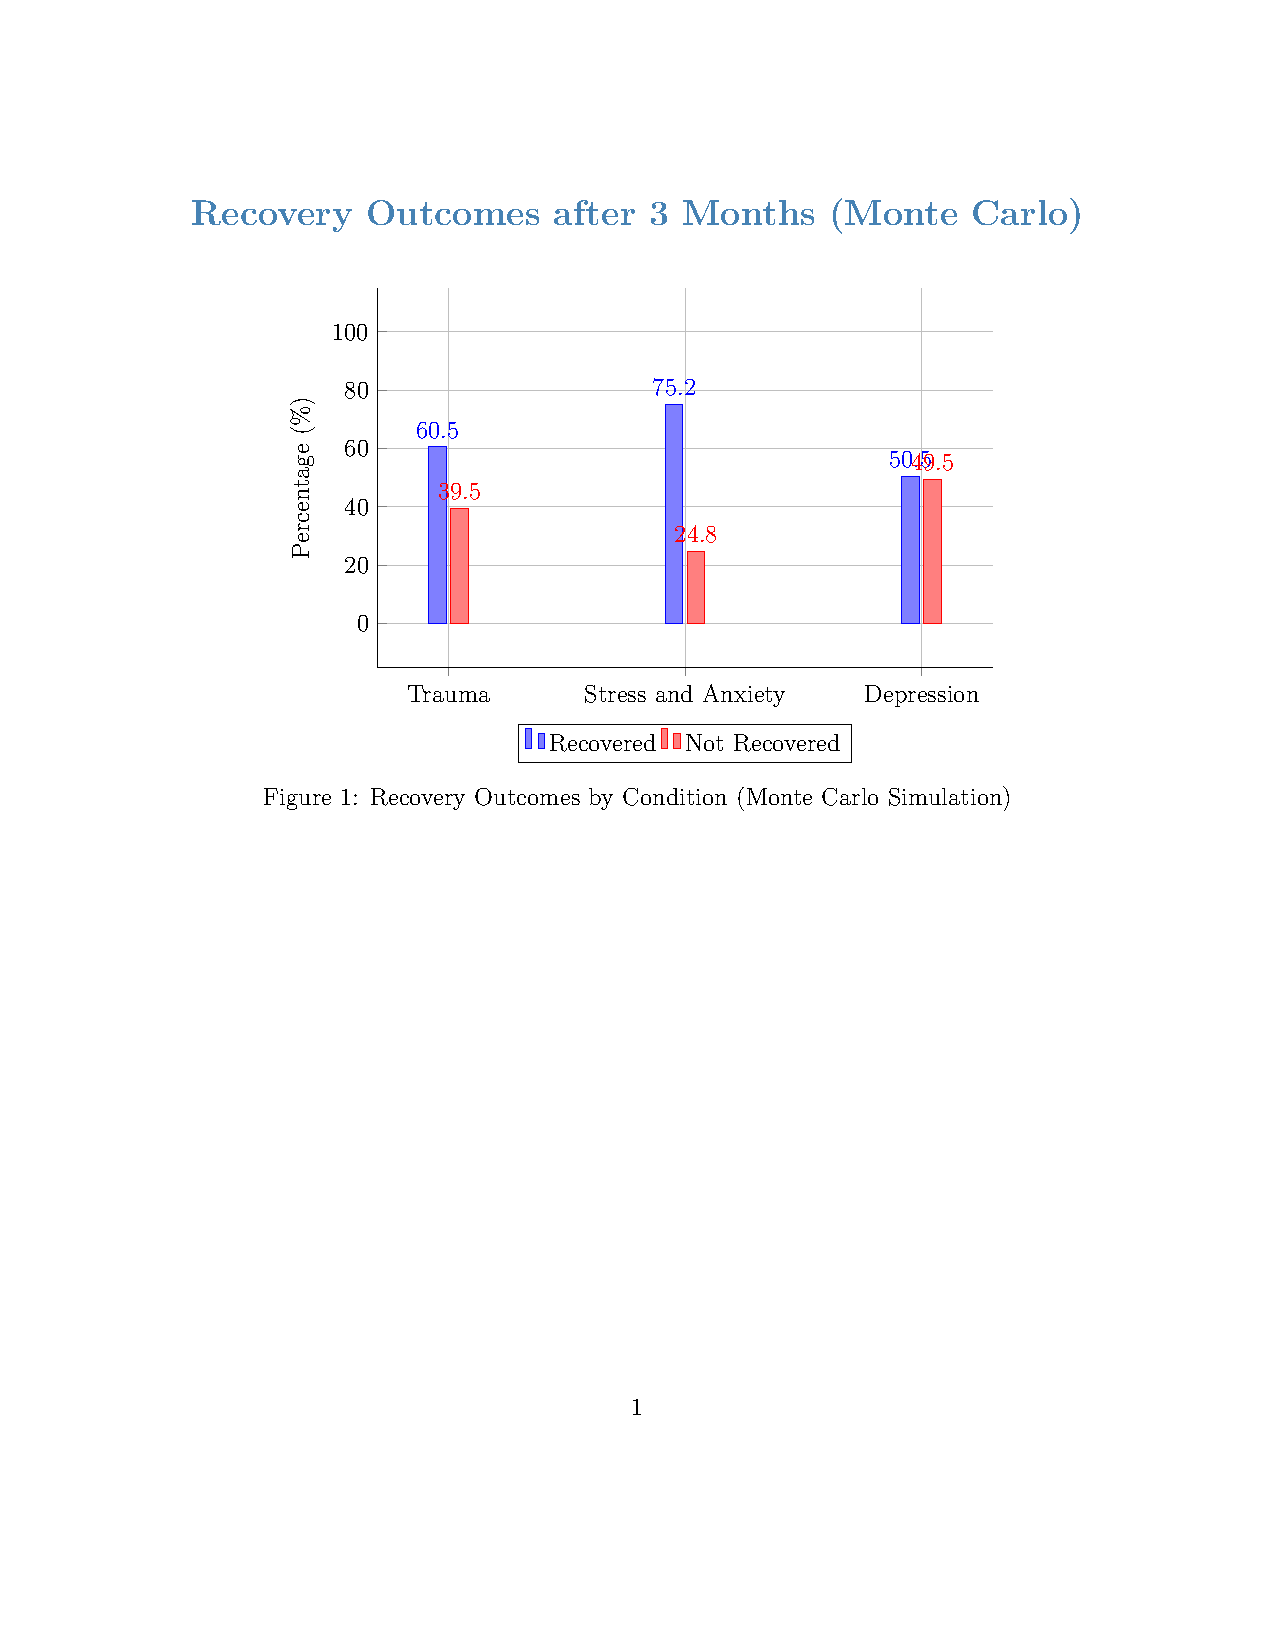
\includegraphics[width=0.8\textwidth]{fig.pdf}
\end{center}

\section*{Conclusion}
The simulation suggests that tailored support protocols yield varying recovery rates. 
Students suffering from stress and anxiety have the highest recovery probability, 
while depression shows the lowest. Continued support and monitoring are recommended.

\end{document}



import numpy as np
import pandas as pd
from scipy.stats import chi2_contingency
# SETTINGS
n_students = 100
n_simulations = 1000
# Generate students
np.random.seed(1234)

# Randomly assign categories
conditions = np.random.choice(
    ['Trauma', 'Stress and Anxiety', 'Depression'],
    size=n_students
)

# Assign doctors
doctors = []
for cond in conditions:
    if cond == 'Trauma':
        doctors.append('Dr_A_Trauma')
    elif cond == 'Stress and Anxiety':
        doctors.append('Dr_B_Stress_Anxiety')
    elif cond == 'Depression':
        doctors.append('Dr_C_Depression')

students_df = pd.DataFrame({
    'ID': range(1, n_students + 1),
    'Condition': conditions,
    'Doctor': doctors
})

print("Initial Distribution:")
print(students_df['Condition'].value_counts())

# Simulate outcomes
results = []

for sim in range(n_simulations):
    for idx, row in students_df.iterrows():
        rand = np.random.rand()
        if row['Condition'] == 'Trauma':
            recovered = 'Recovered' if rand < 0.60 else 'Not_Recovered'
        elif row['Condition'] == 'Stress and Anxiety':
            recovered = 'Recovered' if rand < 0.75 else 'Not_Recovered'
        elif row['Condition'] == 'Depression':
            recovered = 'Recovered' if rand < 0.50 else 'Not_Recovered'
        results.append({
            'ID': row['ID'],
            'Condition': row['Condition'],
            'Doctor': row['Doctor'],
            'Simulation': sim + 1,
            'Outcome': recovered
        })

results_df = pd.DataFrame(results)

# Tabulate outcomes
summary = pd.crosstab(
    results_df['Condition'],
    results_df['Outcome'],
    margins=True,
    normalize='index'
) * 100

print("\nRecovery Outcomes (%):")
print(summary)

# Chi-square test
contingency = pd.crosstab(
    results_df['Condition'],
    results_df['Outcome']
)

chi2, p, dof, expected = chi2_contingency(contingency)

print("\nChi-square Test:")
print(f"Chi2 Statistic: {chi2:.4f}")
print(f"p-value: {p:.4f}")

# Save to Excel
results_df.to_excel("results_python_simulation.xlsx", index=False)
print("\nResults exported to 'results_python_simulation.xlsx'")

